\documentclass[a4paper,11pt,twoside]{report}
% KOMPILOWAĆ ZA POMOCĄ pdfLaTeXa, PRZEZ XeLaTeXa MOŻE NIE BYĆ POLSKICH ZNAKÓW

% -------------- Kodowanie znaków, język polski -------------

\usepackage[utf8]{inputenc}
\usepackage[MeX]{polski}
\usepackage[T1]{fontenc}
\usepackage[english,polish]{babel}

\usepackage{subfiles}
\usepackage{graphicx}
\usepackage{caption}
\usepackage{float}
\usepackage{footnote}
\usepackage{multirow}
\usepackage{array}
\usepackage{enumitem}
\usepackage{seqsplit}
\graphicspath{
    {../screens}
    {../diagrams}
    {../api}
}


\usepackage{amsmath, amsfonts, amsthm, latexsym} % głównie symbole matematyczne, środowiska twierdzeń

\usepackage[final]{pdfpages} % inputowanie pdfa
%\usepackage[backend=bibtex, style=verbose-trad2]{biblatex}

\usepackage{commath} % różne komendy ułatwiające pisanie wyrażeń matematycznych --- warto zapoznać się z dokumentacją: https://ctan.gust.org.pl/tex-archive/macros/latex/contrib/commath/commath.pdf

\usepackage[hidelinks]{hyperref} % dla hiperlinków, m.in url , odnośników do równań, czy bibliografii --- opcja hideboxes usuwa prostokąty wokół kiperlinków

% ---------------- Marginesy, akapity, interlinia ------------------

\usepackage[inner=20mm, outer=20mm, bindingoffset=10mm, top=25mm, bottom=25mm]{geometry}


\linespread{1.5}
\allowdisplaybreaks

\usepackage{indentfirst} % opcjonalnie; pierwszy akapit z wcięciem
\setlength{\parindent}{5mm}


%--------------------------- ŻYWA PAGINA ------------------------

\usepackage{fancyhdr}
\pagestyle{fancy}
\fancyhf{}
% numery stron: lewa do lewego, prawa do prawego
\fancyfoot[LE,RO]{\thepage}
% prawa pagina: zawartość \rightmark do lewego, wewnętrznego (marginesu)
\fancyhead[LO]{\sc \nouppercase{\rightmark}}
% lewa pagina: zawartość \leftmark do prawego, wewnętrznego (marginesu)
\fancyhead[RE]{\sc \leftmark}

\renewcommand{\chaptermark}[1]{
\markboth{\thechapter.\ #1}{}}

% kreski oddzielające paginy (górną i dolną):
\renewcommand{\headrulewidth}{0 pt} % 0 - nie ma, 0.5 - jest linia


\fancypagestyle{plain}{% to definiuje wygląd pierwszej strony nowego rozdziału - obecnie tylko numeracja
  \fancyhf{}%
  \fancyfoot[LE,RO]{\thepage}%

  \renewcommand{\headrulewidth}{0pt}% Line at the header invisible
  \renewcommand{\footrulewidth}{0.0pt}
}



% ---------------- Nagłówki rozdziałów ---------------------

\usepackage{titlesec}
\titleformat{\chapter}%[display]
  {\normalfont\Large \bfseries}
  {\thechapter.}{1ex}{\Large}

\titleformat{\section}
  {\normalfont\large\bfseries}
  {\thesection.}{1ex}{}
\titlespacing{\section}{0pt}{30pt}{20pt}
%\titlespacing{\co}{akapit}{ile przed}{ile po}

\titleformat{\subsection}
  {\normalfont \bfseries}
  {\thesubsection.}{1ex}{}


% ----------------------- Spis treści ---------------------------
\def\cleardoublepage{\clearpage\if@twoside
\ifodd\c@page\else\hbox{}\thispagestyle{empty}\newpage
\if@twocolumn\hbox{}\newpage\fi\fi\fi}


% kropki dla chapterów
\usepackage{etoolbox}
\makeatletter
\patchcmd{\l@chapter}
  {\hfil}
  {\leaders\hbox{\normalfont$\m@th\mkern \@dotsep mu\hbox{.}\mkern \@dotsep mu$}\hfill}
  {}{}
\makeatother

\usepackage{titletoc}
\makeatletter
\titlecontents{chapter}% <section-type>
  [0pt]% <left>
  {}% <above-code>
  {\bfseries \thecontentslabel.\quad}% <numbered-entry-format>
  {\bfseries}% <numberless-entry-format>
  {\bfseries\leaders\hbox{\normalfont$\m@th\mkern \@dotsep mu\hbox{.}\mkern \@dotsep mu$}\hfill\contentspage}% <filler-page-format>

\titlecontents{section}
  [1em]
  {}
  {\thecontentslabel.\quad}
  {}
  {\leaders\hbox{\normalfont$\m@th\mkern \@dotsep mu\hbox{.}\mkern \@dotsep mu$}\hfill\contentspage}

\titlecontents{subsection}
  [2em]
  {}
  {\thecontentslabel.\quad}
  {}
  {\leaders\hbox{\normalfont$\m@th\mkern \@dotsep mu\hbox{.}\mkern \@dotsep mu$}\hfill\contentspage}
\makeatother



% ---------------------- Spisy tabel i obrazków ----------------------

\renewcommand*{\thetable}{\arabic{chapter}.\arabic{table}}
\renewcommand*{\thefigure}{\arabic{chapter}.\arabic{figure}}
%\let\c@table\c@figure % jeśli włączone, numeruje tabele i obrazki razem


% --------------------- Definicje, twierdzenia etc. ---------------


\makeatletter
\newtheoremstyle{definition}%    % Name
{3ex}%                          % Space above
{3ex}%                          % Space below
{\upshape}%                      % Body font
{}%                              % Indent amount
{\bfseries}%                     % Theorem head font
{.}%                             % Punctuation after theorem head
{.5em}%                            % Space after theorem head, ' ', or \newline
{\thmname{#1}\thmnumber{ #2}\thmnote{ (#3)}}%  % Theorem head spec (can be left empty, meaning `normal')
\makeatother

% ----------------------------- POLSKI --------------------------------

\theoremstyle{definition}
\newtheorem{theorem}{Twierdzenie}[chapter]
\newtheorem{lemma}[theorem]{Lemat}
\newtheorem{example}[theorem]{Przykład}
\newtheorem{proposition}[theorem]{Stwierdzenie}
\newtheorem{corollary}[theorem]{Wniosek}
\newtheorem{definition}[theorem]{Definicja}
\newtheorem{remark}[theorem]{Uwaga}



% ----------------------------- Dowód -----------------------------

%\makeatletter
%\renewenvironment{proof}[1][\proofname]
%{\par
%  \vspace{-12pt}% remove the space after the theorem
%  \pushQED{\qed}%
%  \normalfont
%  \topsep0pt \partopsep0pt % no space before
%  \trivlist
%  \item[\hskip\labelsep
%        \sc
%    #1\@addpunct{:}]\ignorespaces
%}
%{%
%  \popQED\endtrivlist\@endpefalse
%  \addvspace{20pt} % some space after
%}
%
%\renewcommand{\qedhere}{\hfill \qedsymbol}
%\makeatother





% -------------------------- POCZĄTEK --------------------------


% --------------------- Ustawienia użytkownika ------------------

\newcommand{\tytul}{System do zdalnej pracy w środowisku graficznym wykorzystujący maszyny wirtualne QEMU z akceleracja sprzętową}
\renewcommand{\title}{Environment for remote work with Graphical User Interface using QEMU virtual machines with hardware acceleration}
\newcommand{\type}{inżyniers} % magisters, licencjac
\newcommand{\supervisor}{dr inż. Marek Kozłowski}



\begin{document}
\sloppy


\includepdf[pages=-]{titlepage/titlepage}


% ------------------ STRONA Z PODPISAMI AUTORA/AUTORÓW I PROMOTORA ------------------


\thispagestyle{empty}\newpage
\null

\vfill

\begin{center}
  \begin{tabular}[t]{ccc}

    ............................................. & \hspace*{100pt} & ............................................. \\
    podpis promotora                              & \hspace*{100pt} & podpisy autorów
  \end{tabular}
\end{center}


% ---------------------------- ABSTRAKTY -----------------------------
% W PRACY PO POLSKU, NAPIERW STRESZCZENIE PL, POTEM ABSTRACT EN
%
%	Streszczenie powinno zajmować 1 stronę, (czcionką 12)
%

{ \fontsize{12}{14} \selectfont
\begin{abstract}

  \begin{center}
    \tytul
  \end{center}
  Streszczam.

  Lorem ipsum dolor sit amet, consetetur sadipscing elit, sed diam nonumyeirmod tempor invidunt ut labore et dolore magna aliquyam erat, sed diamvoluptua. At vero eos et accusam et justo duo dolores et ea rebum. Stet clita kasd gubergren, no sea takimata sanctus est Lorem ipsum dolor sit amet.\\

  \noindent \textbf{Słowa kluczowe:} slowo1, slowo2, ...
\end{abstract}
}

\null\thispagestyle{empty}\newpage

{\selectlanguage{english} \fontsize{12}{14} \selectfont
  \begin{abstract}

    \begin{center}
      \title
    \end{center}
    Konieczne jest załączenie wypełnionego oświadczenia o autorstwie pracy. By tego dokonać, skan (w formacie PDF) należy umieścić w folderze \emph{scans} i nazwać go, np.  oswiadczenie\_o\_autorstwie\_pracy.pdf (w przypadku innej nazwy lub umieszczenia w innym folderze, konieczne jest adekwatne zmodyfikowanie ścieżki w komendzie je załączającej --- patrz fragment kodu OŚWIADCZENIA.\\

    \noindent \textbf{Keywords:} keyword1, keyword2, ...
  \end{abstract}
}

\null\thispagestyle{empty}\newpage
% --------------------- OŚWIADCZENIA -----------------------------------------

%
%	KONIECZNE JEST ZAŁĄCZENIE WYPEŁNIONEGO SKANU OŚWIADCZENIA O AUTORSTWIE PRACY. SKAN (W FORMACIE PDF) NALEŻY UMIEŚCIĆ W FOLDERZE scans I NAZWAĆ GO, NP.  oswiadczenie_o_autorstwie_pracy.pdf (W PRZYPADKU INNEJ NAZWY, LUB UMIESZCZENIA W INNYM FOLDERZE KONIECZNE JEST ADEKWATNE ZMODYFIKOWANIE ŚCIEŻKI W PONIŻSZEJ KOMENDZIE.
%
%	komenda załączająca oświadczenie o autorstwie pracy
%
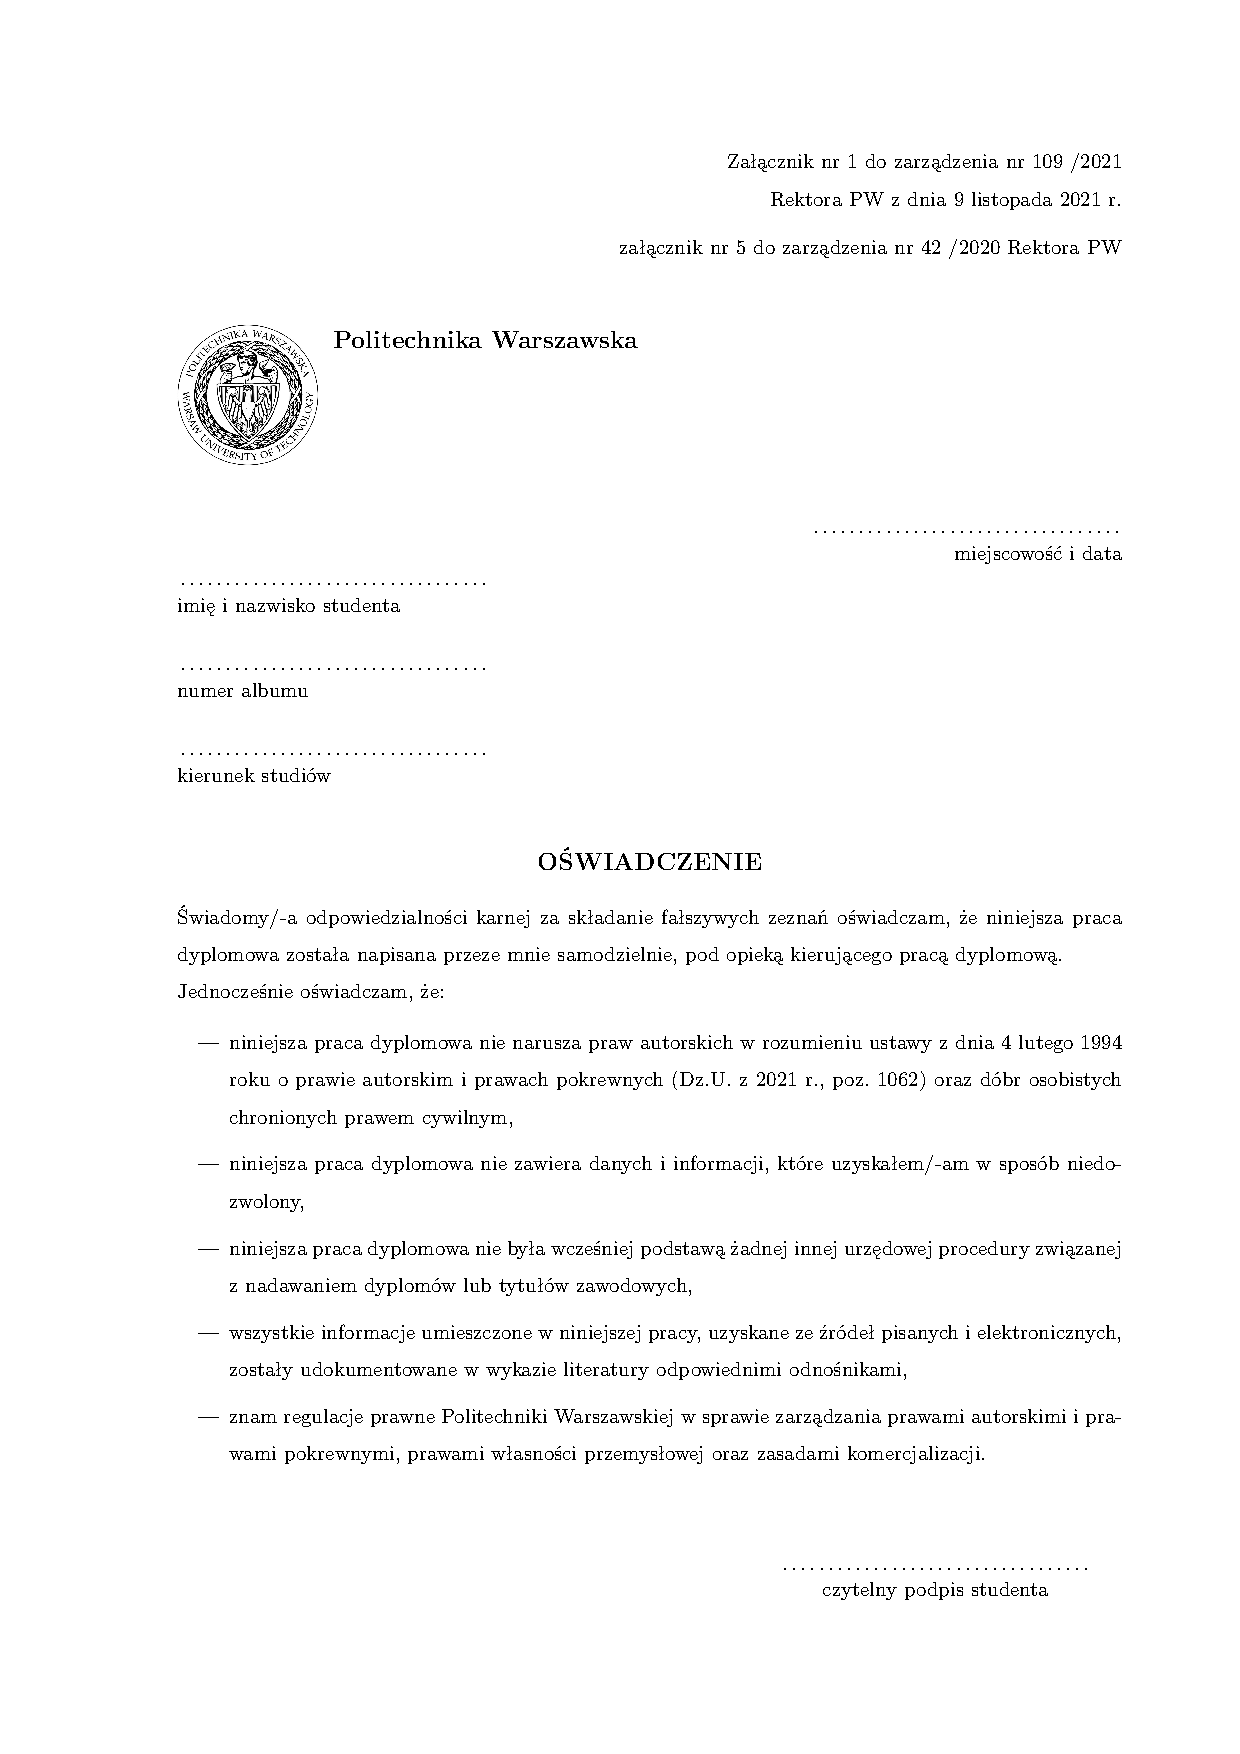
\includepdf[pages=-]{scans/oswiadczenie-o-autorstwie-pracy}
\null\thispagestyle{empty}\newpage

% opcjonalne oświadczenie
%
%	komenda załączająca owiadczenie o udzieleniu licencji
%
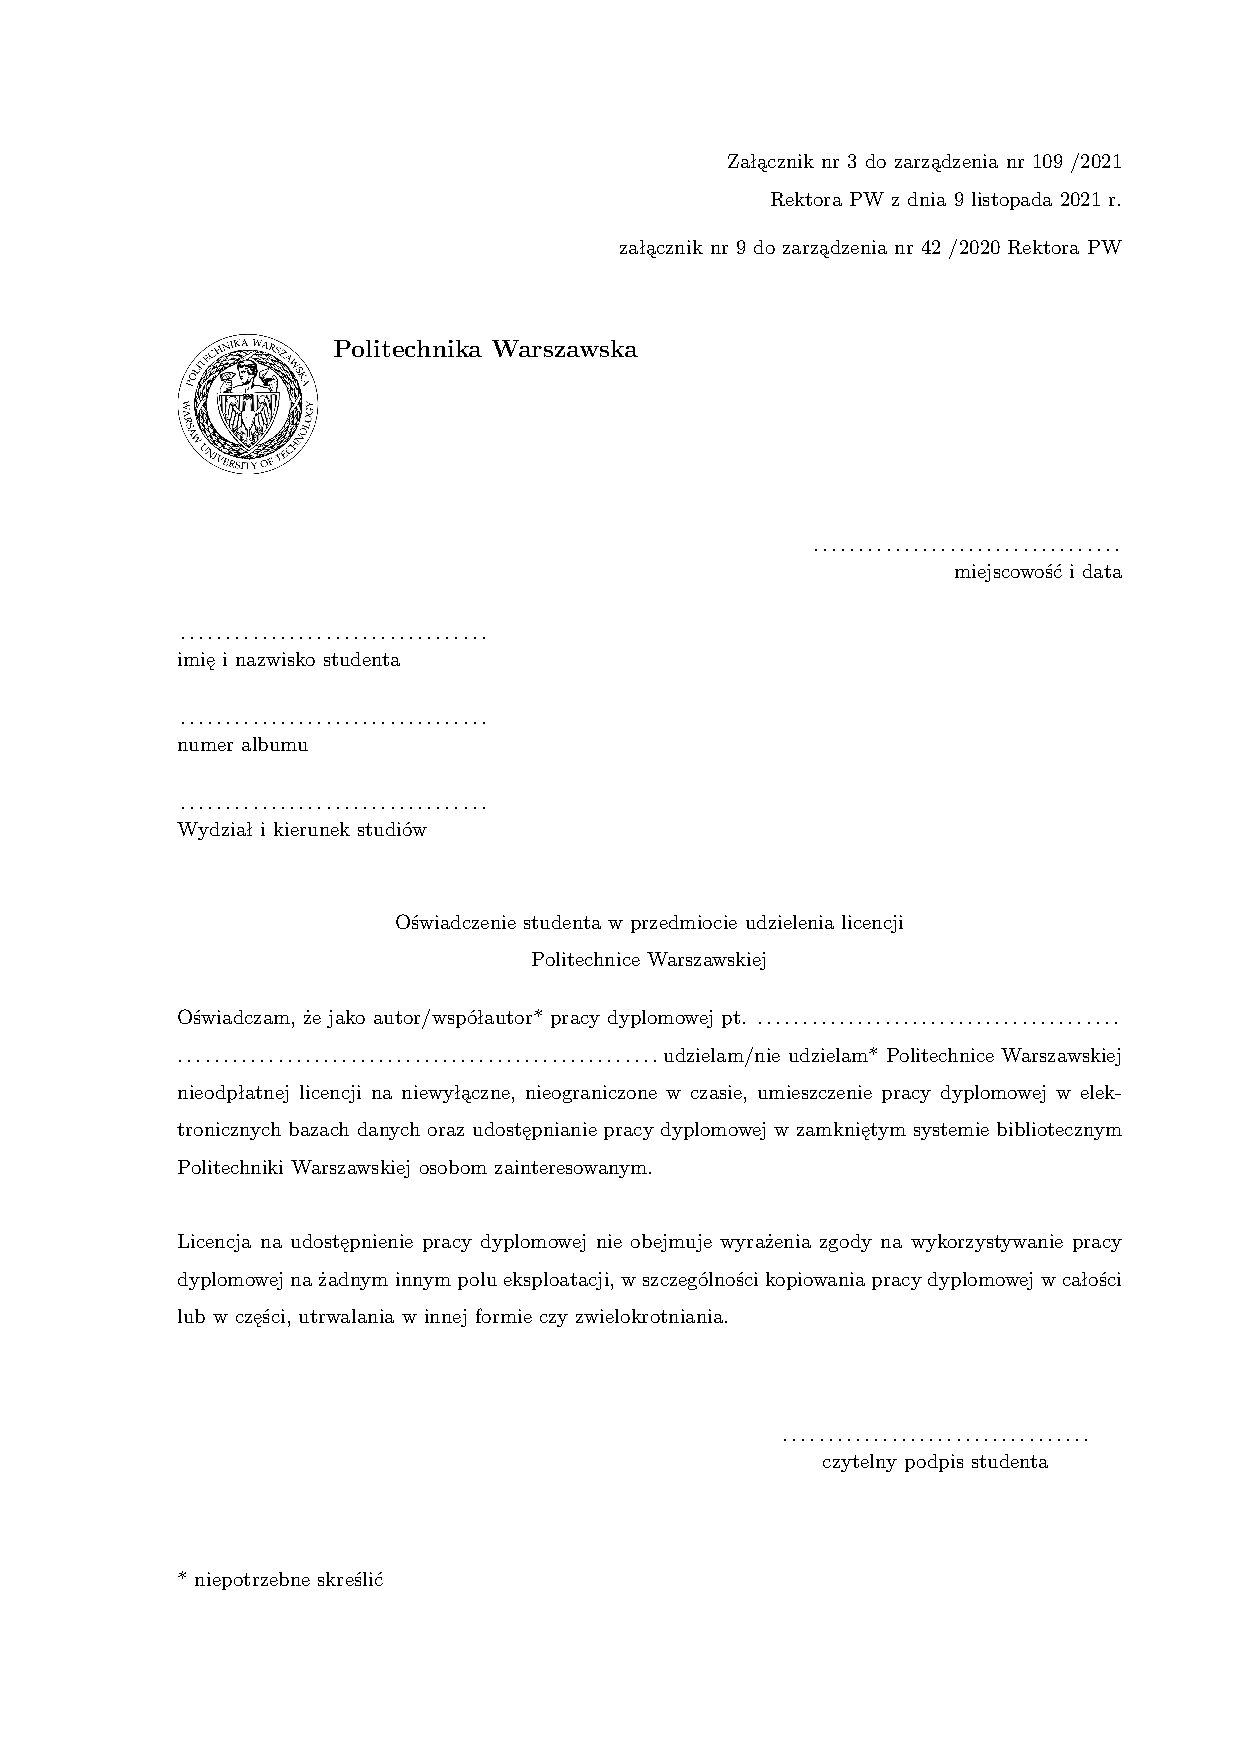
\includepdf[pages=-]{scans/oswiadczenie-o-udzieleniu-licencji}
%
%	pliki .texowe odpowiadające powyższym plikom PDF znajdują się w folderze 3. declarations
%
\null\thispagestyle{empty}\newpage

% ------------------- 4. Spis treści ---------------------
\pagenumbering{gobble}
\tableofcontents
\thispagestyle{empty}

\newpage % JEŻELI SPIS TREŚCI MA PARZYSTĄ LICZBĘ STRON, ZAKOMENTOWAĆ
% ALBO JAK KTOŚ WOLI WTEDY DWIE STRONY ODSTĘPU, DODAĆ \null\newpage

% -------------- 5. ZASADNICZA CZĘŚĆ PRACY --------------------
\null\thispagestyle{empty}\newpage
\pagestyle{fancy}
\pagenumbering{arabic}
\setcounter{page}{11} % JEŻELI Z POWODU DUŻEJ ILOŚCI STRON W SPISIE TREŚCI SIĘ NIE ZGADZA, TRZEBA ZMODYFIKOWAĆ RĘCZNIE

\chapter{Wstęp}
% \markboth{}{Wstęp}
% \addcontentsline{toc}{chapter}{Wstęp}

%Rozdział wstępny
\subfile{sections/wstep.tex}

\chapter{Opis rozwiązania}

%Opis rozwiązania - plan po zrozumieniu problemu
\subfile{sections/opis-rozwiazania.tex}

\chapter{Analiza rozwiązania}

%Analiza rozwiązania - analiza wykonanego rozwiązania
\subfile{sections/analiza-rozwiazania.tex}

\chapter{Podsumowanie}

% Podsymowianie - co osiągneliśmy i co dalej
\subfile{sections/podsumowanie.tex}

% \begin{table}% Koniecznie label po caption, inaczej jest zła numeracja
%   \caption[Opis skrócony]{Opcje dodatkowe dla tabel i rysunków}
%   \label{opcje}
%   \centering
%   \begin{tabular}{|c|p{0.8\textwidth}|}
%     \hline
%     symbol opcji & efekt                                                                                                                                                               \\ \hline
%     \texttt{h}   & bez przemieszczenia, dokładnie w miejscu użycia (uzyteczne w odniesieniu do niewielkich wstawek); raczej niestosowane                                               \\
%     \texttt{t}   & na górze strony; stosowane najczęściej                                                                                                                              \\
%     \texttt{b}   & na dole strony                                                                                                                                                      \\
%     \texttt{p}   & na stronie zawierającej wyłącznie wstawki                                                                                                                           \\
%     \texttt{!}   & ignorując większość parametrów kontrolujacych umieszczanie wstawek, przekroczenie wartosci, których może nie pozwolić na umieszczanie nastepnych wstawek na stronie \\ \hline
%   \end{tabular}
% \end{table}

% W tablicy \ref{opcje} znajdują się opcje dodatkowe otoczeń \texttt{table} i \texttt{figure}.

% \begin{figure}[h!]

%   \begin{center}
%     \setlength{\unitlength}{1mm}

%     \begin{picture}(40, 30)
%       \put(20,1){\line(0,1){20}} % linia

%       % dół
%       \put(20,1){\circle*{2}}
%       \put(25,1){0}

%       % góra
%       \put(20,21){\circle*{2}}
%       \put(25,21){1}
%     \end{picture}

%   \end{center}
%   \caption{Przykładowy rysunek, który można wygenerować w \LaTeX -u}
% \end{figure}

% -------------------- 6. Bibliografia -----------------------
% Bibliografia leksykograficznie wg nazwisk autorów
% Dla ambitnych - można skorzystać z BibTeX-a
\subfile{sections/bibliografia.tex}

\thispagestyle{empty}
\pagenumbering{gobble}


% --- 7. Wykaz symboli i skrótów - jeśli nie ma, zakomentować
\chapter*{Wykaz symboli i skrótów}

\begin{tabular}{cl}
  nzw.           & nadzwyczajny      \\
  *              & operator gwiazdka \\
  $\widetilde{}$ & tylda
\end{tabular}
\\
Jak nie występują, usunąć.
\thispagestyle{empty}


% ----- 8. Spis rysunków - jeśli nie ma, zakomentować --------
\listoffigures
\thispagestyle{empty}


% ------------ 9. Spis tabel - jak wyżej ------------------
\renewcommand{\listtablename}{Spis tabel}
\listoftables
\thispagestyle{empty}


% 10. Spis załączników - jak nie ma załączników, to zakomentować lub usunąć

\chapter*{Spis załączników}
\begin{enumerate}
  \item Załącznik 1
  \item Załącznik 2
  \item Jak nie występują, usunąć rozdział.
\end{enumerate}
\thispagestyle{empty}


\end{document}
